\documentclass{article}

\usepackage{amssymb}
\usepackage{amsthm}
\usepackage{amsmath}
\usepackage{graphicx}
\usepackage{mathptmx}
\usepackage{lipsum}  % for sample text
\usepackage[T1]{fontenc}
\usepackage{textcomp}
\usepackage{dirtytalk}
\usepackage{listings}
% \usepackage{subfigure}
\usepackage{subcaption}


%include these lines if you want to use the LaTeX "theorem" environments
\newtheorem{theorem}{Theorem}[section]
\newtheorem{definition}[theorem]{Definition}
\newtheorem{claim}[theorem]{Claim}
\newtheorem{lemma}[theorem]{Lemma}
\newtheorem{corollary}[theorem]{Corollary}
% \newenvironment{claim}[1]{\par\noindent\underline{Claim:}\space#1}{}
% \newenvironment{claimproof}[1]{\par\noindent\underline{Proof:}\space#1}{\hfill $\blacksquare$}

%include lines like this if you want to define your own commands 
%to save typing
\newcommand{\PROOF}{\noindent {\bf Proof}: }
\newcommand{\REF}[1]{[\ref{#1}]}
\newcommand{\Ref}[1]{(\ref{#1})}
\newcommand{\dt}{\mbox{\rm   dt}}
\newcommand{\phat}{\hat{p}}


 \usepackage{setspace}
 \onehalfspacing
 \newtheorem{mytheorem}{Theorem}
 \numberwithin{mytheorem}{subsection} % important bit


\begin{document}

	\title{The Penney Ante Problem}
	\author{Saleh Hindi}

	\maketitle

	\section{Introduction}
		Imagine a two player game where
		each player is assigned a sequence, for example THTH and HTHH, and a coin is flipped until either player sees their sequence.
		The first player to see their sequence appear wins.
		Given two sequences, which sequence is expected to come first in the
		sequence of coin flips? What is the probability of a certain player winning? Although these two
		questions sound similar, the result is that in our example,
		the expected number of turns for sequence A to appear is 20 and for B it is 18. However, surprisingly, the probability
		of A winning is 9/14 while the probability of B winning is 5/14. Additionally the game has the property
		that for any sequence A chooses, B can always find a sequence that has a higher probability of winning.
		These counterintuitive results are the core of the Penney Ante problem, discovered by Walter Penney
		\cite{gardner}. My thesis will study this problem through three approaches based in Markov chains, martingales,
		and a counting approach.

	\section{Definitions and Notation}
		Let $X_t$ be a random variable for $t \geq 1$, and let $(X_t)$ be a stochastic sequence of letters chosen uniformly and
		randomly from a $q$-letter alphabet. The statespace of $(X_t)$ will be denoted $\Omega$ with each state equal to an $x \in \Omega$. In the case of a coin, $q=2$ and $(X_t)$ represents the sequence of coin flips. Let $A=a_1a_2...a_n$ and $B=b_1b_2...b_n$ be sequences
		of $n$ letters chosen from the $q$-letter alphabet. We say
		sequence $A$ or $B$ wins if it is the first sequence to appear within $(X_t)$ or more precisely, $A$ or $B$ wins if it is the lowest $i$ such that $A = a_1a_2...a_n = X_iX_{i+1}...X_n$ or $B = b_1b_2...b_n = X_iX_{i+1}...X_n$. Let $\tau_A$ and $\tau_B$ be random variables denoting
		the number of turns required for $A$ or $B$ to appear. We denote
		the probability of $A$ winning as $P(\tau_A < \tau_B)$ and we denote the expected time for sequence
		$A$ and $B$ to appear as $E(\tau_A)$ and $E(\tau_B)$. This notation will be used throughout of the paper. 

		We can use Conway's algorithm to find $P(\tau_A < \tau_B)$ and $E(\tau_A)$. Conway devised an algorithm for computing these two values which has been described as an algorithm that "cranks out the answer as if by magic" \cite{gardner}. The algorithm is as follows,

		\begin{theorem}(Conway's Algorithm \cite{gardner})
		Given two sequences of length $n$, $A$ and $B$, we find the correlation in base 2, $AB_2$, by the following algorithm:
		\begin{enumerate}
		\item loop through integers 1, 2, ..., n,
		\item At every ith iteration we look at the ith through nth digits of A and compare
		   it to the 1st through the (n-i)th digits of B.
		\item If these subsequences are equal, the ith digit in the binary representation is 1 but 0 otherwise.
		\end{enumerate} 

		The binary number of $AB_2$
		is then converted to a decimal number, $AB$. Once we find $AA$, $AB$,
		$BA$, and $BB$, the probability that A precedes B is
		$$P(\tau_A < \tau_B) = \frac{AA - AB}{(BB - BA) + (AA - AB)} $$
		Furthermore, 
		$$E(\tau_A) = 2AA $$ 
		\end{theorem}

		Throughout the paper we will use $A = HTHT$ and $B = HTHH$ as an example. If we plug this example into Conway's formula we get that $E(\tau_{A}) = 20$ and $E(\tau_{B}) = 18$.

		\begin{figure}[h]
			\begin{center}
				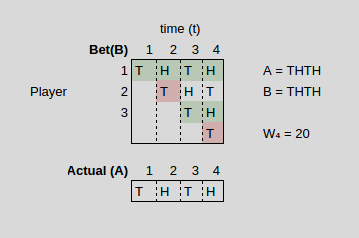
\includegraphics[width=2.5in]{AA}
			\end{center}
		
			\caption{Calculation of AA. $E(\tau_A) = 20$.}
		\label{fig}
		\end{figure}

		% An interesting property of $F(z)$ is that it is rational in this case so we can write it as $F(z) = \frac{P(z)}{Q(z)}$ for $Q(z) \neq 0$ and coprime $P(z)$, $Q(z)$. From $F(z)$ being rational, we can derive the main combinatoric result which will let us count the number subsequences of a sequence which are not equal to the sequence and thus the number of subsequences which are equal to the sequence.

		Finally, we define nontransitivity. In this context, a game is nontransitive if for any sequence A, player B can choose a sequence B such that $P(\tau_A < \tau_B)$. In later sections we will see that the Penney ante game is nontransitive for $n \geq 4$. In general nontransitivity is....




	\section{Martingales}
		\subsection{Introduction}
			We can study the Penney ante problem using a mathematical object called a martingale. A martingale is a stochastic sequence such that at any time, the expected value of the random variable is the same. We call a martingale with an expected value of 0 a fair game. More precisely,

			\begin{definition}[\cite{li}]
				A {\em martingale} is a stochastic sequence $(X_t)$ such that for any
				integer $k$ and for any finite expected value $E(|X_k|)$, $$E(X_{k+1} | X_1, ..., X_k) = X_k$$		
			\end{definition}

		    Let's define a martingale representing the Penney Ante game. Given a stochastic sequence of coin flips $(X_t)$, and for each $t$, define $W_t$, assuming $W_0=0$,
		    \[ W_{t+1}=\begin{cases} 
		      W_{t} + 2^t & \text{if $X_t$ = some value that we are betting on}\\
		      0 & \text{otherwise} 
			  \end{cases} \]

		    We can reformulate the Penney ante problem into a game found in Grinstead \cite{grinstead}. We will see that the sequence representing the total winnings in this game, $W_t$, is a martingale \cite{grinstead}. We can then find $E_{\varnothing}(\tau_{B})$ with the help of Doob's convergence theorem, and then $E_A(\tau_{B})$, and using some probability we find that $P(\tau_{B} < \tau_{A})$. This method allows us to prove that $E(\tau_A) < E(\tau_B)$ does not imply $P(\tau_A < \tau_B) > \frac{1}{2}$ and it also reveals the inner workings of Conway's algorithm. 

		    Given sequences $A$ and $B$, imagine at each turn $t$, a player joins the game and bets 1 choosing to play double or nothing until either they lose or the sequence $B$ is found. On a player's $i$th turn, the player bets on the $i$th letter of $B$ appearing while in fact the $t$th letter of $A$ actually appears. The number of turns in the game is equal to the length of $A$. We will denote this betting strategy, betting on $B$ while $A$ appears, $AB$. At each turn if the player's bet matches the actual outcome, they double their money, otherwise they lose all of their money and stop playing. On each subsequent turn, another player joins the game and also bets $AB$. At each turn, $W_t$ is the earnings of all the players for time $t$. Note in this game the case where $B$ is a substring of $A$ is trivial because... \cite{grinstead} 

		    ***How does this formulation represent the original Penney ante problem...

		\subsection{Example}
			Consider $A = B = HTH$ as an example. Figure \ref{fig} demonstrates the game in a table. At each turn, a new player enters the game and bets on $B$. Player $i$'s bet at time $t$ is denoted by the $i$th row in the $t$th column in the table. The actual letter appearing is in the 'Actual' table below. The green denotes a match while red denotes a mismatch and thus the stopping of betting for that player. 
			\begin{figure}[h]
				\begin{center}
					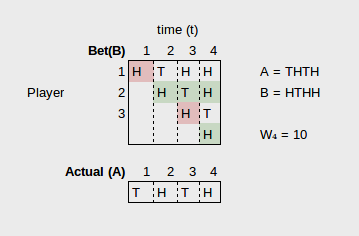
\includegraphics[width=2.5in]{AB}
				\end{center}
			
				\caption{Calculation of $W_3$ for $A = B = HTH$.}
				\label{fig}
			\end{figure}

			Note the repetitive pattern of the table. A table very similar to this will be generated in Conway's algorithm for determining the expected waiting times. 

		\subsection{Expected Winning Times and Probability of B Winning}
		    To prove that $E(\tau_B) = BB$, we must first show that $W_t$ is a martingale.

			\begin{claim}
				$W_t$ is a martingale.
			\end{claim}

			\begin{PROOF}
				From our earlier definition of a martingale we know that $W_t$ is martingale if for each $k$, $E(W_{k+1} | W_1,W_2,...,W_k) = W_k$. Informally, we can see at each time $t$, the value of each of the gambler's winnings double or go to zero with a .5 chance each way. That means the expected value of each gambler's winnings at time $t+1$ is the value of their winnings at time $t$. This seems to indicate that the expected value of $W_{t+1}$ is just the value of $W_t$, making it a martingale. More formally, given a stochastic sequence of coin flips $(X_t)$, and for $t > 0$, we can define $W_t$ as, 
			    \[ W_{t+1}=\begin{cases} 
			      W_{t} + 2^t & \text{if $X_t$ = some value that we are betting on}\\
			      0 & \text{otherwise} 
				  \end{cases} \]

				 Once we choose an $X_t$ to bet on, there is a .5 chance of the bet winning. So $E(W_{t+1}) = \frac{1}{2}(W_t + 2^t) + \frac{1}{2}(0)$. Find the right formula for Wt so this part works out*** \qed
			\end{PROOF}

			Now we can find $E_{\varnothing}(\tau_{B})$. Note that the final payout of the game occurs at time $t=\tau_{B}$, when sequence $B$ fully appears. The random variable $\tau_B$ is a stopping time. (Should I prove that $\tau_{B}$ is a stopping time?). First we need Doob's Martingale Convergence Theorem which states that if SOME QUANTITY INVOLVING A RANDOM VARIABLE*** converges to zero then the expected value of the random variable at time $t=\tau_B$ is equal to it's expected value at the stopping time. Formally,

			\begin{theorem}(Doob's Martingale Convergence Theorem)
				Let $W_t$ be a martingale and $\tau_B$ a stopping time. If,
				$$\liminf\limits_{k\rightarrow \infty} \int_{\tau_B > k} |W_k|dP = 0$$
				then $\{W_1, W_{\tau_B}\}$ is a martingale and $E(W_{\tau_B}) = E(W_1)$.
			\end{theorem}

			As stated earlier, $W_t$ is indeed a martingale and $\tau_B$ is a stopping time. So we need to show $\liminf\limits_{k\rightarrow \infty} \int_{\tau_B > k} |W_k|dP = 0$. Because XXX we know that $W_{\tau_{AB}} = BB - \tau_{AB}$.

			$$E(W_{\tau_{AB}}) \leq BB + E(\tau_{AB}) < \infty$$

			Let $Aw_k B$ represent the sequence XXX followed by XXX. Then for $\tau_{AB} > k$,
			\begin{equation}
			\begin{split}
			W_k & \leq (Aw_k B) + k \\
			    & \leq BB + \tau_{AB} \\
			\end{split}
			\end{equation}

			This implies that,
			$$\lim_{k\rightarrow \infty} \int_{\tau_{AB}} |W_k|dP \leq \lim_{k\rightarrow \infty} \int_{\tau_{AB}} (BB + \tau_{AB}) dP = 0$$

			So now we are able to use Doob's convergence theorem to find that,
			$$E(W_{\tau_{AB}}) = E(W_0) = AB$$

			From the fact that $W_{\tau_{AB}} = BB - \tau_{AB}$, it's true that,
			$$E(\tau_{AB}) = BB - AB$$.

			***Remember $\tau_{AB}$ is the random variable representing the time it takes for $B$ to appear starting with $A$.

			***The payout at this time, $W_{\tau_{B}}$ is equal to $BB$, the amount won from betting on $B$ while sequence $B$ appears. So $E_{\varnothing}(\tau_{B}) = BB$. Now for $AB$, the first $k$ tosses (where $k$ is the length of A), the gamblers collectively make $AB$, ie $W_k = AB$. The total amount the gamblers make at $t = \tau_{B}$ is thus $BB - BA$ so $E_A(\tau_{B}) = BB - BA$. \cite{grinstead}.

			Now what is $P(\tau_{B} < \tau_{A})$? Note that for two random variables, $X$, $Y$, $P(X > Y) = \frac{E(X)}{E(X) + E(Y)}$ \cite{grinstead}. So, $$P(\tau_{B} < \tau_{A}) = \frac{E_A(\tau_{B})}{E_A(\tau_{B}) + E_B(\tau_{A})} = \frac{AA - AB}{(BB - BA) + (AA - AB)}$$

	\section{Markov Chains}
		As stated earlier, $E(\tau_A) < E(\tau_B)$ does not imply $P(\tau_A < \tau_B) > \frac{1}{2}$. To prove and understand this result, we will construct a Markov chain. A Markov chain is a stochastic sequence $(X_t)$ that has the probability that each state of the chain occurs -- ie each $X_k$ -- is based solely on the previous state, $X_{k-1}$ for all $k > 1$. Markov chains allow the sequence to be represented by a graph with all the possible states of the sequence as vertices. Edges connecting vertices denote probabilities between that a state will occur after another state. More formally,

		\begin{definition}[\cite{textbook}]
			A {\em Markov chain} is a stochastic sequence such that
			$$P(X_{k+1} = x | X_1, X_2, ..., X_k) = P(X_{k+1} = x  | X_k)$$
			That is, the probability that each $x \in \Omega$ occurs given the entire history of
			previous states is only dependent on the most recent event. Denote the probability
			that $P(X_{k+1}=y|X_k=x)$ as $P(x,y)$. The matrix $P = P(x,y)$ for all $x,y \in \Omega$ is called the transition matrix of $(X_t)$.
		\end{definition}

		The Penney ante game can be represented as a Markov chain because each sequence of coin flips, for example $X_4=HTHT$, depends only on the previous state $X_3$ and not the entire history of states. We can use Markov chains to find $E(\tau_A)$ and $P(\tau_A < \tau_B)$ by writing a system of equations for the probability and expected value of each state which will be done next section. 


		Using Markov chains, we can construct a system of equations for the expected waiting time to win and probability of a sequence winning. Let $p_{x}$ denote the probability sequence $A$ of length $n$ wins given that $x\in\Omega$ has occured. To find $p_\emptyset$, the probability of A winning given nothing has happened, we can construct a system of $n+1$ equations for each $X_t$ composed of probabilities times of reaching $x$ from $y$. Assuming $x$ -- $y$ means $P(x,y) > 0$,

		% \textasciitilde for a tilde
		$$p_x = \sum_{y - x} P(x,y) p_y$$

		In this game where $q=2$, each sum will have two terms since there will only be at most two states $x$ that are reachable from each state $y$. Similarly, we can find the expected value with this method but with a small change. Let $E_x$ denote the time to win given $x$ has occurred. Then we can write a system of $n+1$ equations,

		$$E_x = \sum_{y - x} P(x,y) (1 + E_y)$$

		% Note the we add 1 to $E_y$ because.... 

		\begin{figure}[h]
			\begin{center}
				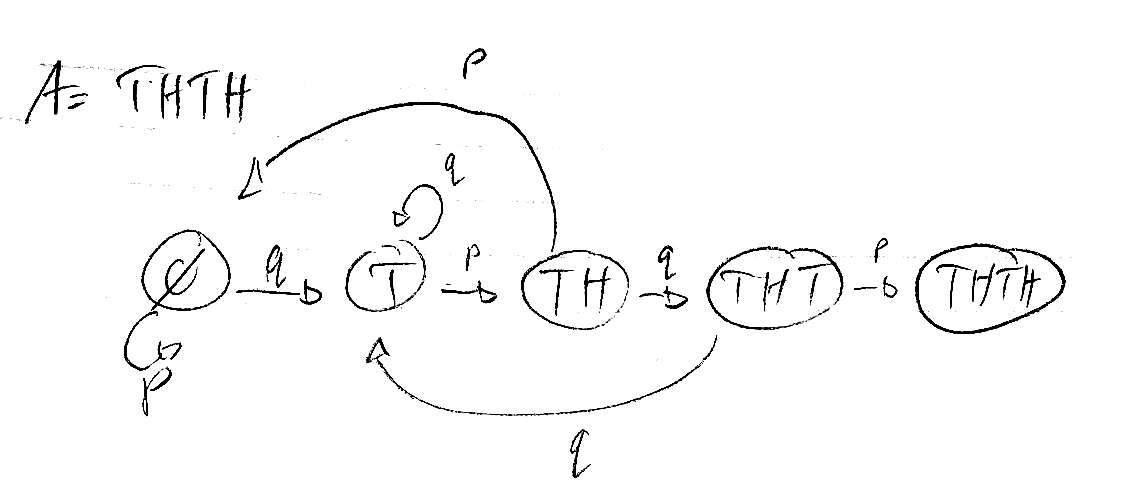
\includegraphics[width=4.0in]{GameOfA}
			\end{center}
		
			\caption{The graph of $\Omega_A$}
			\label{perfect_fig}
		\end{figure}
		\begin{figure}[h]
			\begin{center}
				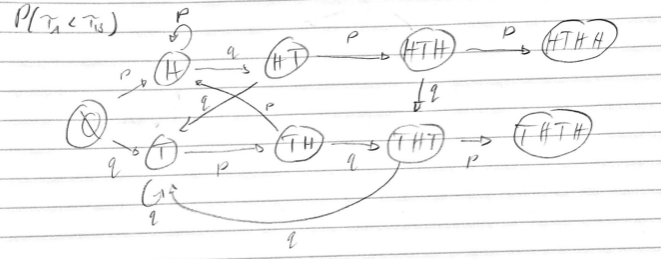
\includegraphics[width=4.0in]{winning}
			\end{center}
		
			\caption{The graph of the game (What is the best way to draw graphs on a computer? This method looks very sloppy...)}
			\label{perfect_fig}
		\end{figure}

		As an example, let $A = THTH$ and $B = HTHH$. Although not all possible sequences have the property that, $E(\tau_A) < E(\tau_B)$ while $P(\tau_A < \tau_B) > \frac{1}{2}$, this particular example goes against our intuition so it is worthwhile to look at. As stated in the introduction, $E(\tau_A)$ is 20, $E(\tau_B)$ is 18, and $P(\tau_A > \tau_B) = \frac{9}{14}$. As a sanity check, we should check that the three methods described in the previous section give the same answer for $P(\tau_A > \tau_B)$ and $E(\tau_B)$. 

		With the Markov chain approach, we can directly construct the transition matrix $P$. The $P$ for $A=THTH$ is,
		\begin{equation} 	
			P= \left(
			\begin{array}{ccccc}
			 0.5 & 0.5 & 0 & 0 & 0 \\
			 0 & 0.5 & 0.5 & 0 & 0 \\
			 0 & 0 & 0.5 & 0.5 & 0 \\
			 0 & 0 & 0 & 0.5 & 0.5 \\
			 0 & 0 & 0 & 0 & 1 \\
			\end{array}
			\right)
		\end{equation}
		Where each $i$th column or row represents $\emptyset$, $T$, $TH$, $THT$, or $THTH$ accordingly which indicate how close A is to winning. For $B = HTHH$, the states would be $\emptyset$, $H$, $HT$, $HTH$, and $HTHH$.

		Using this matrix, we construct the systems of equations for the probability as follows,
		\begin{equation} 	
		\begin{split}
		p_{\emptyset} & = \frac{1}{2} p_{THT} \\
		p_{T} & = \frac{1}{2} p_{TH} + \frac{1}{2} p_{\emptyset} \\
		p_{TH} & = \frac{1}{2} p_{THT} + \frac{1}{2} p_T \\
		p_{THT} & = \frac{1}{2} p_{THTH} + \frac{1}{2} p_{TH} \\
		p_{THTH} & = 1 \\
		\end{split}
		\end{equation}

		Using Mathematica (how should I include the code? Directly in the paper or as a footnote?) we find that $p_{THTH} = \frac{9}{14}$. (Insert Mathematica Code) For the expected value we have,
		\begin{equation} 	
		\begin{split}
		E_{\emptyset} & = \frac{1}{2} (1 + E_{THT}) \\
		E_{T} & = \frac{1}{2} (1 + E_{TH}) + \frac{1}{2} (1 + E_{\emptyset}) \\
		E_{TH} & = \frac{1}{2} (1 + E_{THT}) + \frac{1}{2} (1 + E_{THT}) \\
		E_{THT} & = \frac{1}{2} (1 + E_{THTH}) + \frac{1}{2} (1 + E_{TH}) \\
		E_{THTH} & = 1 \\
		\end{split}
		\end{equation}

		The calculation for B is omitted because it is essentially the same. Using the same Mathematica code we find that $E_{THTHT} = 20$. Thus concludes the calculation using the Markov chain approach. Conway's algorithm gives us the same result. 

		Consider $A = THTH$. The calculation $AA$ is as follows,   
		\begin{lstlisting}[escapechar=\%]
		1010 
		%\underline{THTH}%
		THTH
		 THTH
		  THTH 
		   THTH 
		\end{lstlisting}

		The binary number 1010 in decimal is 9 so $E(\tau_{THTH}) = 18$ and $P(\tau_A < \tau_B) = \frac{9}{14}$.

		
	\section{Generating Function}
		And finally, we will be using a combinatoric method for finding $E(\tau_A)$ based around finding the generating function for the number of $x \in \Omega$ which contain $A$ as a substring. For a given sequence $A$, let $f(n)$ denote the number of sequences of length $n$ that do not contain $A$ as a subsequence. A generating function in general can be formally defined as,
		\begin{definition}[\cite{enumerate}]
			Given any sequence $(X_t)$, we define its generating function $F(z)$ to be
			$$F(z) = \sum_{n=0}^\infty f(n) z^{-n}$$
			where $z$ is an unknown variable.
		\end{definition}

		Now that we have the correlation $AB$, we can also use the generating function approach the compute the desired values. The probability that $A$ does not appear in the first $n$ coin tosses is $f(n)2^{-n}$. The expected number of coin tosses until $A$ appears is,
		$$\sum_{n=0}^\infty f(n) 2^{-n} = F(2)$$
		From 
		$$F(z) = \frac{zAA_z}{1+(z-q)AA_z}$$
		we can get that $F(2) = 2AA$. \cite{enumerate} \cite{gardner}

		The probability that A does not appear in the first $n$ coin tosses is $f(n)2^{-n}$ \cite{enumerate}. The expected number of coin tosses can be derived from these facts and will involve a number called the correlation of two strings, denoted $AB$. The correlation $AB$ will be better defined later when outlining Conway's algorithm. Conway devised a "magic algorithm" which let us compute $AB$ which will be used to find the expected winning time and the probability of A winning. This operation $AB$ has a careful connection to the $AB$ defined in the betting strategy. The correlation will give us the expected number of coin tosses until $A$ appears and it is also used to model the above gambling game. The connection between the two $AB$'s will come in a later section.

	\section{Results}
		\subsection{Martingales}
			The betting game described earlier creates a martingale process, $(W_t)$. Notice how $(X_t)$ and $(W_t)$ derive from the same source of randomness, the independently and uniformly chosen coin flips. Although martingales do not directly give us an easy way to compute the expected waiting time and probability of a sequence winning, it provides a justification to Conway's algorithm. Counting all of the string overlaps of $AB$ is checking the earnings of all the player for partial matches between sequences $A$ and $B$. In binary, moving up each of the digits correspong to the player betting double or nothing. I will go into further detail about martingales and the connection between string enumeration and Conway's algorithm at a future date but know that for now, Conway's algorithm serves as our method of computing the expected waiting time and probability using the martingale approach.


	\section{Future Work}
		In the future I will prove the results stated in the results section. It will also be worthwhile to give a proof of the nontransitivity property which was not stated in the results.

	\begin{thebibliography}{1}
		\bibitem{boyer}
			Boyer, Robert S., and J. Strother Moore. "A Fast String Searching Algorithm." Communications of the ACM 20.10 (1977): 762-72. Web. 
		\bibitem{breen}
			Breen, Stephen, Waterman Michael S., and Zhang Ning. "Renewal Theory for Several Patterns." Journal of Applied Probability 22.1 (1985): 228-34. Web.
		\bibitem{gardner}
			Gardner, Martin. "Mathematical Games: On the Paradoxical Situations That Arise from Nontransitive Relations." Scientific American 10 (1974): 120-25. Print.
		\bibitem{grinstead}
 			Grinstead, Charles M., and J. Laurie Snell. Introduction to Probability. Providence, RI: American Mathematical Society, 1997. Print. 
 		\bibitem{guibas}
			Guibas, L.j, and A.m Odlyzko. "String Overlaps, Pattern Matching, and Nontransitive Games." Journal of Combinatorial Theory, Series A 30.2 (1981): 183-208. Web.
		\bibitem{li}
			Li, Shuo-Yen Robert. "A Martingale Approach to the Study of Occurrence of Sequence Patterns in Repeated Experiments." The Annals of Probability 8.6 (1980): 1171-176. Web.
		\bibitem{nickerson}
			Nickerson, R. S. "Penney Ante: Counterintuitive Probabilities in Coin Tossing." The UMAP Journal 28.4 (2007): 503-32. JSTOR. Web. 8 Sept. 2016. 
		\bibitem{textbook}
			Levin, David Asher, Y. Peres, and Elizabeth L. Wilmer. Markov Chains and Mixing times. Providence, RI: American Mathematical Society, 2009. Print. 
		\bibitem{enumerate}
			Odlyzko, A. M. "Enumeration of Strings." Combinatorial Algorithms on Words (1985): 205-28. Web.
			
	\end{thebibliography}
\end{document}

 